%------------------------------------------------------------------------------
% Template file for the submission of papers to IUCr journals in LaTeX2e
% using the iucr document class
% Copyright 1999-2003 International Union of Crystallography
% Version 1.2 (11 December 2002)
%------------------------------------------------------------------------------
%
\documentclass[preprint]{iucr}              % DO NOT DELETE THIS LINE
                   \def\href#1{\relax}\let\foo\caption
\ifPDF
  \RequirePackage{hyperref}
  \PassOptionsToPackage{pdftex,bookmarksopen,bookmarksnumbered}{hyperref}
  \voffset=-0.5in
\fi
\let\caption\foo

\usepackage{graphicx}
\usepackage[T1]{fontenc}
\usepackage[utf8]{inputenc}
 \usepackage{amsmath}
%\usepackage{eps2pdf}

 \paperprodcode{a000000}      % Replace with production code if known
 \paperref{xx9999}            % Replace xx9999 with reference code if known
 \papertype{IU}               % Indicate type of article
 \paperlang{english}          % Can be english, french, german or russian
 \journalcode{S}             % Indicate the journal to which submitted
 \journalyr{2017}
 \journalreceived{\relax}
 \journalaccepted{\relax}
 \journalonline{\relax}

\begin{document}                  % DO NOT DELETE THIS LINE

 \title{Real-time diffraction contrast tomography data reduction}
 \shorttitle{GPU decompression and integration of CBF images}

 \cauthor[a]{J.}{Kieffer}{jerome.kieffer@esrf.fr}{}
 \author[a]{S.}{Petitdemange}
 \author[a]{T.}{Vincent}
  
 \aff[a]{ESRF, The European Synchrotron, CS40220, 38043 \city{Grenoble}
 Cedex 9, \country{France}}
 \shortauthor{Kieffer & al.}


\keyword{Powder diffraction}
\keyword{Diffraction imaging}
\keyword{Pilatus detector}
\keyword{Image compression}
\keyword{Azimuthal integration}
\keyword{pyFAI}
\keyword{FabIO}
\keyword{silx}



\maketitle                        % DO NOT DELETE THIS LINE

\begin{synopsis}
Benchmark of the data-analysis pipeline for XRD-CT. CBF byte-offset
decompression on GPU.
\end{synopsis}

\begin{abstract}

Diffraction imaging is an X-Ray imaging method which uses the cristallinity
information (cell parameter, orientation ) as signal to create an image pixel
per pixel:
a pencil beam is raster-scanned onto a sample and the (powder) diffraction
signal is recorded by a large area detector.
With the flux provided by third generation synchrotrons and the speed of
hybrid pixel-detector, the acquisition speed of those experiments is now 
limited by the transfer rate to the local storage as the data reduction can
hardly be performed in real time.

This contribution presents the benchmarking of a typical data
analysis pipeline for a diffraction imaging experiment like the one performed at
ESRF ID15a and proposes some disruptive techniques to decode CBF images using the
computational power of graphics cards to be able to perform data reduction in
real-time.
\end{abstract}


\section{Introduction}

Since all major third-generation synchrotrons are undergoing upgrades
to provide brighter sources \cite{ESRF-EBS, S8U} the same
flux of photon will be available soon in much smaller beam. 
Two types of experiments will benefit the most from this improved
X-ray source: coherence diffraction experiments and raster-scanning
experiments.

X-Ray diffraction computed tomography (hereafter XRD-CT, Figure \ref{diff_tomo}),
\cite{XRDCT} is one of the raster scanning experiments where a pencil beam is 
scanned onto a sample.
The volumetric information is obtained by rotating the sample in the X-ray beam
to generate the sinogram.
The diffraction signal, scattered over a large solid angle is recorded by
an area detector and saved as a stack of images.
Those images are azimuthal averaged into powder diffraction patterns with the
intensity given as a function of either the diffraction angle ($2\theta$) or the scattering
vector $q=4 \pi sin (2\theta/2)/\lambda$.
The sinogram is built, pixel per pixel, by storing this pattern as a function of
the sample position: translations and rotation.
The tomogram is finally reconstructed from the back-projection of the sinogram.  

\begin{figure}
\label{diff_tomo}
\begin{center}
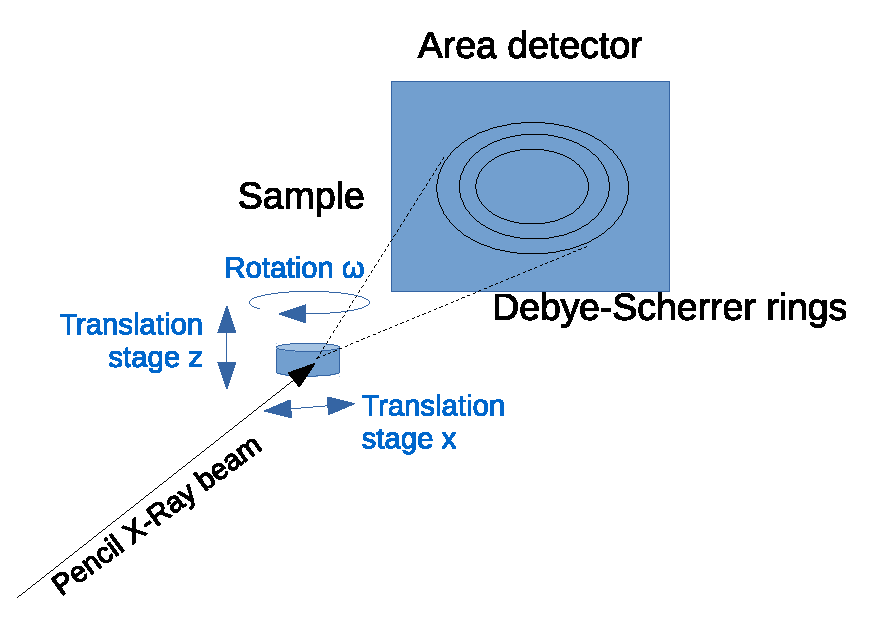
\includegraphics[width=15cm]{Diffraction_imaging.eps}
\caption{Scheme of a X-Ray diffraction tomography setup where the
sample can be translated and rotated in front of a pencil beam. 
The Debye-Scherrer rings formed by the diffraction of crystallites are collected
by an area-detector, integrated into a powder diffraction pattern and
assembled to create a sinogram, which is computationally back-projected to build
the tomogram.}
\end{center}
\end{figure}

 
It turns out that the current detectors are already fast enough to fill the temporary
storage and data analysis workflows cannot cope with the pace imposed by
modern detectors \cite{GigaFRoST}: data analysis \emph{is} the limiting factor
for the whole experiment.
This work focuses on the performance optimization of the data reduction
pipeline for the cases where the reduction is simply an azimuthal
regrouping of input images.
More complex analysis are possible (and often desirable) but the target of this
work is online data analysis so the analysis will be restricted to simple ones.

We will focus in the second section on the setup of the Materials beamline
(ID15a) of the ESRF  \cite{id15a} and perform a complete benchmarking of the
data analysis pipeline used. 
This will highlight various bottle-necks in the data-analysis chain.
To address the image decompression bottle-neck, different parallelization
schemes have been developed and are presented in section 3. 

\section{X-ray diffraction imaging: data analysis pipeline}

\subsection{Beamline hardware}

\subsubsection{Pilatus3 2M CdTe detector:}

The ID15a beamline at ESRF uses mainly a Pilatus3 2M detector with a 1000 $\mu
m$ CdTe sensor, manufactured by Dectris \cite{pilatus}. 
The detector is made-up of 8x3 Pilatus modules (100 kilopixel each).
Unlike Silicon-based sensors, there are two Cd-Te wafers bump-bound to every
Pilatus-module, with a gap of 3 pixels between the wafers.
The gaps between the Piltus modules are the same as the Silicon-based
detectors, i.e. 7 pixels vertically and 17 pixel horizontally.

This detector is sold with a detector-PC which is in charge of compressing and
saving the images on the network. 
This detector-PC comes with a 10 Gbit/s network card and is directly connected
to the data analysis server.

The detector is advertised to operate at 250 frames per second.
Each frame has 2.4 megapixels, stored as 32-bits integers (the dynamic range is
only 20 bits).
At full speed, the raw (uncompressed) stream represents hence 19.2 gigabits per
second to transfer. 
Compression is hence mandatory to transfer the acquired data through the 10
gigabits per second network interface.
Dectris uses the CIF binary format (CBF) \cite{cbf} for Pilatus detectors
with byte-offset compression which provides a compression factor close to 4x. 
An alternative compression scheme used in the novel Eiger detector is the LZ4
but the compression factor is much less, around 2x (and variable, depending on
the signal of the detector) which makes this option un-applicable for operating
the Pilatus detector continuously over an extended period of time.

\subsubsection{The data analysis computer}
(Figure \ref{computer}) acts as a NFS (network file server) server over RDMA
(remote direct memory access) for optimal performance with the detector and is
directly connected to the GPFS (general parallel file-system)
storage cluster \cite{gpfs}.
This data analysis computer has two processors Intel Xeon E5-2643 v3, each with 
6 cores and  20 MB of cache, and 128 GB of memory. 
There is additionally two 10-gigabit network cards, a fast Intel P3700
solid-state drive (SSD), and a Nvidia Titan-X graphics card, all connected on
the PCI-express bus.

\begin{figure}
\label{computer}
\begin{center}
\includegraphics[width=15cm]{lid15agpu1.eps}
\caption{Data-analysis computer with the main interconnections and their
associated bandwidth}
\end{center}
\end{figure}


\subsection{Processing of diffraction imaging experiment}

The pre-processing for diffraction imaging experiments is typically the
azimuthal integration of the whole image with some mask. 
The code snippet of Appendix-\ref{sequentialsnippet} is a typical example:
each image is read, integrated in a 1D profile and saved in a HDF5 file (here not
following the Nexus \cite{nexus} convention for the sake of concision in this example).

This code snippet is written in Python \cite{python} programming language and
uses some external libraries:
\begin{itemize}
  \item {H5Py}: the binding for the HDF5 library in Python \cite{h5py}
  \item{FabIO}: a library for reading most of the X-ray images format
  \cite{fabio}
  \item{PyFAI}: the library which performs the azimuthal
  integration from 2D images to 1D profile \cite{pyFAI}. 
\end{itemize}

The function ``process'' described in this code snippet has been used for
profiling the application (i.e., measuring the bottle-neck in performance).
The input dataset is composed of 1202 images in CBF-format coming from an actual
experiment on ID15a stored on the SSD.
One should distinguish two cases: when data is only available on the
solid-state disk and when it is available in the cache of the
operating system.
The total amount of raw-data is 3 gigabytes, so only the first read can be
considered as a ``cold-start'', subsequent reads actually benefit from
the cache of the operating system and should be considered as ``hot-start''.
To be able to profile in ``cold-start'', the disk has been un-mount and re-mounted
to flush all caches.
Each measurement has been performed five times and the results are reported in
Table \ref{Performances}.  Only the median framerate  with the median absolute
deviation to this median have been reported in frames per second (or Hertz).

The first and the third (resp. second and fourth) line report the performance
in cold- and hot-start.
This allows us to evaluate the actual read time per frame from the SSD
drive which is 4 milliseconds (resp. 5 ms).

As a consequence, it is impossible to process images at 250 frames per
second from this SSD as it is not possible to read the (compressed) data
at the required pace.
There is an emerging technology (3D X-Point technology by Intel) for replacing
NAND cells in SSDs which looks promising and should offer
lower latency for acting as a cache for the raw data. 
As of today, those drives are not yet available in capacities large
enough for replacing the memory for the kind of temporary storage needed for
beamline application.

As online data analysis has to rely on data ``living in memory'' and not
read from any drive, the 128 gigabytes of memory available on the computer
represents a cache of about three minutes of experiment time and thus the data
analysis pipeline has to keep the pace of the experiment. 
Profiling ``precisely'' the data-analysis program is hence of crucial
importance.

\subsection{Profiling of the data-analysis pipeline}

The snippet of code from Appendix-\ref{sequentialsnippet} presented previously has been run in a profiler to
measure how much time is spent in every part of the code for a reference
dataset of 1202 compressed images.
The code executes on this reference dataset in 43 s and the
three most time consuming parts are: the azimuthal integration (29 s), the
byte-offset decompression (4.9 s) and the checksum calculation (4.7 s).
The checksum verification is optional in CBF and may simply be ignored.

The azimuthal integration was originally performed on the processor and could be
off-loaded to the graphics card, which lowers azimuthal integration time to 13 s.
As described in \cite{kieffer_ashiotis-proc-euroscipy-2014}, most of the time
for azimuthal integration on graphics card is spent for the transfer of the raw image to the device.
To speed up the azimuthal integration, the best would be to transfer less data
to the graphics card, i.e the compressed data and decompress them on the GPU.

Remains the bottle-neck of byte-offset decompression \ldots this algorithm will
be described in details in the next section and analyzed. 

\section{Optimizing the decompression of CBF images}

\subsection{Decompression on the processor}

The core idea of the byte-offset compression is to encode only the difference
value between two adjacent pixels and hope this value is small enough to fit in
a 8-bit (signed) integer, i.e in the range -127 to +127.
Larger values are coded with a special value (-128) which indicates an exception
and the subsequent 2 bytes are decoded as a 16-bit integer in little endian
order.
If the value does not fit in a 16-bit integer, a 32-bit exception is
signaled (with value -32768) and the actual value is coded over the next 4 bytes
as a 32 bits little-endian integer.
Hence, each value can be coded with a variable size of 1, 3 (=1+2) or 7 (=1+2+4)
bytes, which makes it very difficult to decompress in a parallel fashion.

Since 2004, processors are running at a maximum speed of about 4GHz.
This means that a serial algorithm like the byte-offset decompression described
previously is running at the same speed today on a high-end computer as it
does on a 13 years-old computer.
Parallelization is the only way to get the processing done faster and a couple
of strategies have been explored and will be presented.

\subsection{Pool of workers strategy} 

A classical strategy in parallel computing is to attribute one type of
computation to a given compute engine.
Azimuthal averaging being already executed on the graphics-card, it is natural
to devote the image decompression to the central processor (CPU).

Unlike lower-end (disk-) drives, where the data access is serialized,
% and the
%best is to have read operations performed in the main thread, then subsequently
%decompression performed in mutiple threads. 
the SSD used in this experiment is interfaced in PCI-express using the NVME
protocol \cite{nvme} which allows thousands of parallel accesses for reading and
writing.
We validated that the performance is actually better when the read step is
performed with multiple threads rather than sequentially on this hardware.

A pool of workers (figure \ref{pool}) is set-up using multiple threads for
reading and decoding the data. 
The number of workers in this pool is the parameter which needs to be
optimized depending on the computer, especially as a function of the
number of processors, of cores, and the amount of cache available.
The list of files to be processed is distributed to the pool of readers via
a parallel queue.
Each worker, which is implemented as a thread, loops over input filenames
it gets from the input-queue.
This queue guarantees that each file is processed once, regardless which worker does the job.
After reading the file and decompressing the data, each worker puts the image
into the output queue.
Later on, azimuthal integration and data saving, using HDF5, is again performed
sequentially. 
As the order of the filenames in the input queue can be different from the order
of the images in the output queue, due to parallel processing, it is important
to propagate the index associated with each filename or frame.

\begin{figure}
\label{pool}
\begin{center}
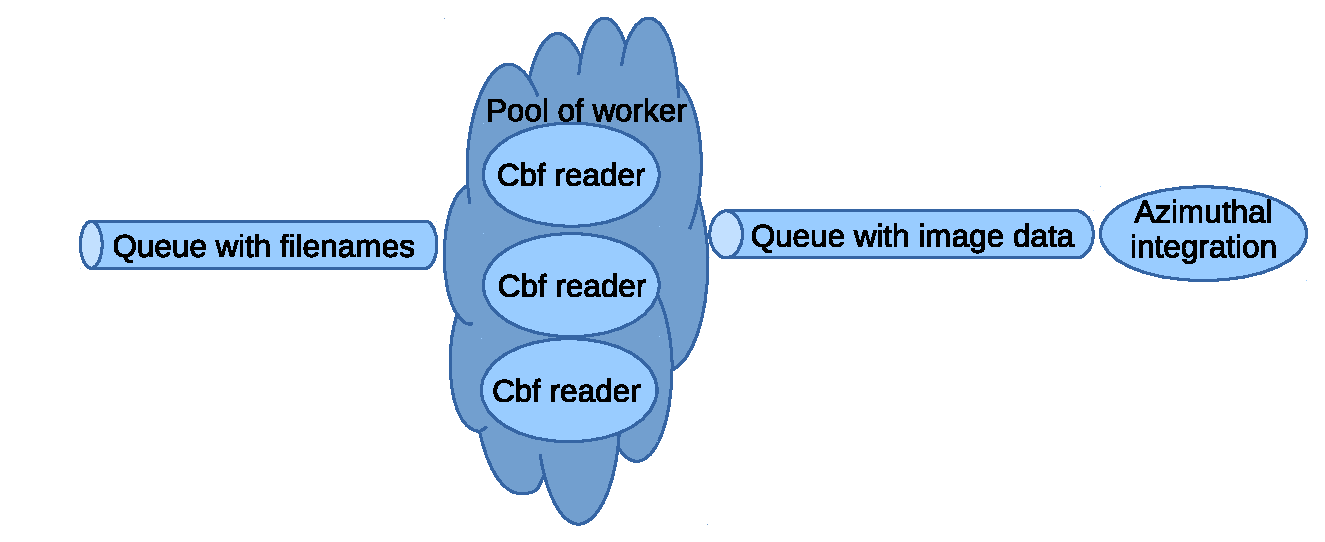
\includegraphics[width=15cm]{pool_of_worker.eps}
\caption{Workflow for the data reduction of a XRD-CT experiment using the pool
of workers pattern.}
\end{center}
\end{figure}


Table \ref{Performances} provides the number of frames processed per second
when processing the sample set of frames and varying the size of the
pool of readers:
1, 2, 3, 4, 6, 12 and 24 workers, all data being already in memory
(hot-start).
This number has to be compared with the framerate of the detector of interest:
250 fps.
The performance of the linear pipeline is given as comparison, in this case the
data can be read from the disk (Intel P3700 SSD, cold-start) or already
available in memory, cached by the operating system (linux).

\begin{table}
\caption{Average performance (in fps) for the azimuthal
integration of 1202 Pilatus3 2M CdTe images saved in CBF format read from
SSD (or from memory) on a dual Xeon E5-2642v3 with a Nvidia Titan-X graphics
card. Median over 5 runs and median deviation to the median.}
\label{Performances}
\vspace{1mm}
\begin{center}
\begin{tabular}{lccccc}
Strategy & Readers & Integrator & Data source & Median speed (fps)  &
deviation (fps)\\
\hline 
Sequential & \textsc{cpu} & \textsc{cpu} & \textsc{ssd} & 28.2 &0.3\\
Sequential & \textsc{cpu} & \textsc{gpu} & \textsc{ssd} & 53.1 &1.4\\
\hline 
Sequential & \textsc{cpu} & \textsc{cpu} & \textsc{mem} & 31.6 &0.9\\
Sequential & \textsc{cpu} & \textsc{gpu} & \textsc{mem} & 74.6 &1.3\\
\hline 
Pool & 1 & \textsc{gpu} & \textsc{mem} & 167 &3\\
Pool & 2 & \textsc{gpu} & \textsc{mem} & 192 &7\\
Pool & 3 & \textsc{gpu} & \textsc{mem} & 155 &5\\
Pool & 4 & \textsc{gpu} & \textsc{mem} & 190 &4\\
Pool & 6 & \textsc{gpu} & \textsc{mem} & 168 &18\\
Pool & 12 & \textsc{gpu} & \textsc{mem} & 121 &4\\
Pool & 24 & \textsc{gpu} & \textsc{mem} & 88 &2\\
\hline 
OpenCL & \textsc{gpu} & \textsc{gpu} & \textsc{mem} & 253 &2\\
\end{tabular}
\end{center}
\end{table}

It is noticeable that the optimal performance is reached with a number of
workers in the pool much lower than the number of cores of the computer, 2 or 4
readers is optimal while the computer has 2x6 cores.
There are multiple reasons for this:
\begin{itemize}
  \item the main thread is also working: it controls the azimuthal
  integrator and the saving of the reduced data in HDF5 format.
  \item the amount of cache of each processor, which is 20 megabytes, has
  to be compared with the 2.5 + 10 megabytes for each frame (encoded + decoded).
  More readers means less CPU-cache for each of them which is detrimental
  to the performance.
  \item Python threads are serialized via the ``global interpreter lock'',
  called \textsc{gil}.
  While most of the processing performed is done in ``no-\textsc{gil}'' section,
  more threads makes it more likely to have them fighting each other
  for acquiring the \textsc{gil}.
\end{itemize}

It is frustrating to have a powerful parallel processor on the
graphics card and seeing the total performance limited by the file-reading
 and decompression which is purely serial.

\subsection{Parallel decompression of CBF images}
 
This section gives an overview of an implementation of the byte-offset
decompression on massively parallel processors like graphics processors
(GPU) using the OpenCL \cite{opencl} programming language.
In those devices, threads are grouped in ``work-groups'' of a given size.
All threads from a work-group perform the same sequence of operations on
different data (in a SIMD way).
This is called a ``kernel'' and looks like a function written in C-language.

Parallel decompression of byte-offset may be divided in the following steps,
each of them being divided into one or two kernels called subsequently:
\begin{itemize}
  \item Search for exceptions in the input stream (marked with the value -128)
  and register them. Other ``normal'' pixel to pixel difference values are simply decoded and stored.
  \item Process all registered sections of contiguous exceptions in parallel to decode them and store their value.
  Here the workgroup size is one, so a single thread is processing a complete
  section of adjacent exceptions and multiple threads are processing multiple
  sections in parallel.
  If a thread starts in the middle of a section of contiguous exceptions,
  it does nothing as this section has to be processed by the thread
  which starts at the beginning of this section of contiguous exceptions.
  \item Compute the cumulative sum of previously stored pixel to pixel difference values.
  This is performed using a ``prefix-sum algorithm'' \cite{scan}.
  \item Compute the position of each value (in the output array)
  using the prefix-sum algorithm: valid pixels position are set to one in the
  input and other remains at zero. This algorithm provides the output pixel
  position for any input position.
  Technically the two prefix-sums are performed simultaneously in our
  implementation for better performance.
  \item Copy the reconstructed values at the proper place in
  the output array, optionally with a conversion to floating point value to
  ease subsequent processing.
\end{itemize} 

The implementation of this algorithm is available as part of the \textit{silx}
\cite{silx} library and will be part of the version 0.7.
While GPUs targeted by this implementation have thousands of
cores, this algorithm remains valid regardless the
number of cores.
Our implementation, based on pyOpenCL \cite{pyopencl}, 
has been validated on different architectures like Nvidia GPUs,
integrated graphics processors (Intel Iris) found in laptops and multi-core
processors (Intel, AMD and Apple OpenCL drivers).

The strength of this approach resides in the limited amount of
data to be sent to the GPU memory, which allows decompression and
integration to be performed on the device without additional
transfer over the PCI-express bus (which is the bottleneck for pyFAI).

The performance of is parallel decompression of CBF images on high-end GPU has
been compared with the serial implementation. 
For large images that do not fit in the cache memory of the
processor (typically for the Pilatus 6M images), the speed-up of this GPU
version is important (10x).
For smaller images, where data fits in the processor cache, the serial
algorithm performs great on CPU, hence the speed-up of the parallel version is
rather limited (+50\%). 
Nevertheless, the combination of the parallel CBF-decompression with azimuthal
integration on the graphics card allows to exceed the 250 frames per second
imposed by the detector as reported on the last line of Table
\ref{Performances}.
Moreover, this parallel implementation naturally benefits from advances in
graphics card processors (i.e., more cores and faster memory):
the same benchmark has been performed on a desktop computer with only one
processor (Xeon 1650v3) instead of 2, with less cache (15MB instead of 20MB),
half the memory (64 GB instead of 128 GB) and a more recent cheaper graphics card
(Nvidia GTX 1080Ti instead of Titan-X).
This desktop computer out-performed the server with more than
300 frames per second for this benchmark.
This parallel algorithm is not only faster than the serial version, it is also
much more stable in performance as the variability (expressed
as the median of absolute difference to the median value) is only of 2 fps on 
the GPU and twice more for the pool of workers pattern. 
The stability of the performance on the GPU can be explained by the dedication
of the graphics card to this calculation.

\section{Outlook}

To be able to inter-connect the decompressed data obtained in the \textit{silx}
library with the azimuthal integrator provided by pyFAI, without transferring the data
back and forth from the device to the processor, the \textit{silx} team implemented a
way to exchange memory objects located on the graphics card between libraries. 
Those results show the validity of the concept and opens the door for
interconnecting different algorithms including image analysis and
tomography algorithms which are available as part of the \textit{silx} library.
In pyFAI, a couple of advanced statistical analysis, recently ported to
OpenCL like median filtering in 2D-integrated data and sigma-clipped
average could also be good candidates for this kind of direct interconnection.

The other strength of this approach is that it hides completely the
complexity of byte-offset decompression with a simple ``decompression object''.
In the GPU-based code snippet (Appendix-\ref{parallelsnippet}) this ``decompression object'' is called ``bo''.
The GPU-base code snippet is equivalent to the sequential one (Appendix-\ref{sequentialsnippet}), it is only a few lines longer and uses the same strategy.

\section{Conclusion}

Processors used for data analysis have hit the power wall more then
a  decade ago.
Since then, no noticeable increase in performance have been seen on
sequential algorithms, causing a bottle-neck in the processing
pipeline for many beamlines, especially the one doing diffraction imaging.
To be able to cope with the stream of data coming from modern detector,
today's fastest SSD drives are not (yet) fast  enough for acting as an
effective cache and the data should best be kept in memory.
Two types of parallelization have been evaluated to speed-up the processing.
The ``pool of workers'' strategy has been evaluated for reading and decoding
different images  in parallel on different cores.
It provides additional performance compared to the serial implementation but
the speed is not, by far, proportional to the number of cores of the computer,
probably due to cache congestion.

The first parallel implementation of the byte-offset decompression
algorithm is also presented.
Leveraging the performance of recent graphics cards, this code allows the reduction
of data for a diffraction imaging experiment performed at full speed with
a Pilatus3 2M detector (250 Hz), in real time.
Moreover this implementation is even faster on newer hardware.

\appendix
\section{Code snippet for sequential decompression and azimuthal integration}

\begin{minipage}{\linewidth}
\label{sequentialsnippet}
\begin{verbatim}
import h5py, fabio, pyFAI

def process(list_of_files, result_file, geometry_file, number_of_bins):
    ai = pyFAI.load(geometry_file)
    with h5py.File(result_file) as result:
        dataset = result.create_dataset("intensities"
                                        (len(list_of_files), number_of_bins),
                                        dtype='float32')
        for index, one_file in enumerate(list_of_files):
            with fabio.open(one_file) as fimg:
                res = ai.integrate1d(fimg.data, number_of_bins)
           dataset[index] = res.intensity
        result['q'] = res.radial
\end{verbatim}
\end{minipage}

\goodbreak

\section{Code snippet for GPU-based decompression and azimuthal integration}

\begin{minipage}{\linewidth}
\label{parallelsnippet}
\begin{verbatim}
import h5py, fabio, pyFAI, os
from silx.opencl.codec.byte_offset import ByteOffset

def process(list_of_files, result_file, geometry_file, number_of_bins):
    ai = pyFAI.load(geometry_file)
    data = fabio.open(list_of_files[0]).data
    res = ai.integrate1d(data, number_of_bins, method="ocl_csr_gpu")
    engine = ai.engines["ocl_csr_integr"].engine
    bo = ByteOffset(os.path.getsize(list_of_files[0]), data.size,
                    ctx=engine.ctx) 
    cbf = fabio.cbfimage.CbfImage()
    with h5py.File(result_file) as result:
        dataset = result.create_dataset("intensities", 
                                       (len(list_of_files), number_of_bins),
                                        dtype='float32') 
        result['q'] = res.radial 
        for index, one_file in enumerate(list_of_files):
            raw = cbf.read(one_file, only_raw=True)
            dec = bo(raw, as_float=True)
            dataset[index] = engine.integrate(dec)[0]
\end{verbatim}
\end{minipage}

\goodbreak

\ack{Acknowledgements:}
This work was carried out on the request of Gavin Vaughan and Marco Di
Michiel, scientists on the Materials diffraction beamline at ESRF (ID15a), who
provided the test dataset composed of 1202 images taken at their beamline with
the Pilatus 2M.
We would like to thank V. Armando Solé, head of Data Analysis Unit and leader
of the \textit{silx} project. 
Finally, we would like to acknowledge the contribution of all other members
of the \textit{silx} project:
Henri Payno, Damien Naudet, Pierre Knobel, Valentin Valls and
Pierre Paleo for the great team work.

\bibliographystyle{iucr}
\bibliography{biblio}

\end{document}
